\documentclass{beamer}

\usepackage[utf8]{inputenc}
\usepackage[T1]{fontenc}

\usepackage{tikz}
\usepackage{microtype}

\usetheme{Median}

\title{Counting to infinity and beyond}
\author{Wenda Zhou}

\begin{document}

\frame{\titlepage}

\section{Ordinals}

\begin{frame}
  \frametitle{Natural numbers}
  \begin{itemize}
  \item<1-> $1$
    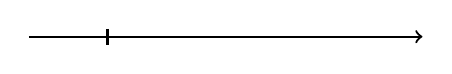
\begin{tikzpicture}
      \draw[thick,->] (0,0) -- (5,0);
      \draw[thick] (1, 0.1) -- (1, -0.1);
    \end{tikzpicture}
  \item<2-> $2$
    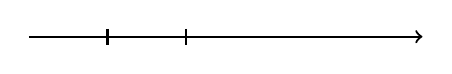
\begin{tikzpicture}
      \draw[thick,->] (0,0) -- (5,0);
      \draw[thick] (1, 0.1) -- (1, -0.1);
      \draw[thick] (2, 0.1) -- (2, -0.1);
    \end{tikzpicture}
  \item<3-> $3$
    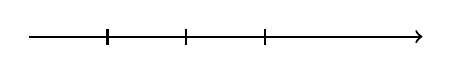
\begin{tikzpicture}
      \draw[thick,->] (0,0) -- (5,0);
      \draw[thick] (1, 0.1) -- (1, -0.1);
      \draw[thick] (2, 0.1) -- (2, -0.1);
      \draw[thick] (3, 0.1) -- (3, -0.1);
    \end{tikzpicture}
  \end{itemize}
\end{frame}

\begin{frame}
  \frametitle{And beyond?}
  \begin{center}
  \Huge What about $\infty$?
  \end{center}
  \pause
  \begin{figure}
    \centering
    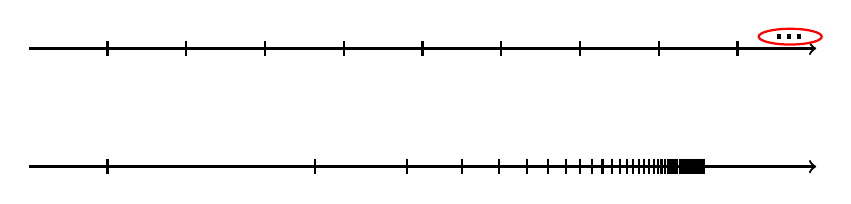
\begin{tikzpicture}
      \draw[thick, ->] (0, 0) -- (10, 0);
      \foreach \x in {1,...,9}
        \draw[thick] (\x, 0.1) -- (\x, -0.1);
      \draw[dotted, ultra thick] (9.5, 0.15) -- (9.85, 0.15);
      \pause
      \visible<3>{\draw[color=red, thick] (9.67, 0.15) ellipse (0.4 and 0.1);}

      \pause
      \draw[thick, ->] (0, -1.5) -- (10, -1.5);
      \foreach \x in {1, ..., 40}
        \draw[thick] ({10 - 9 / sqrt(\x)}, -1.4) -- ({10 - 9 / sqrt(\x)}, -1.6);
    \end{tikzpicture}
  \end{figure}
\end{frame}

\begin{frame}
  \frametitle{Order isomorphisms}

  \begin{figure}
    \centering
    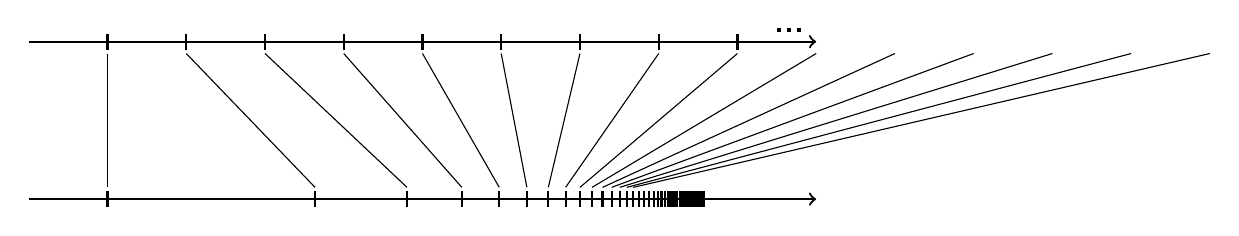
\begin{tikzpicture}
      \draw[thick, ->] (0, 1) -- (10, 1);
      \foreach \x in {1,...,9}
        \draw[thick] (\x, 1.1) -- (\x, 0.9);

      \draw[dotted, ultra thick] (9.5, 1.15) -- (9.85, 1.15);
      \draw[thick, ->] (0, -1) -- (10, -1);

      \foreach \x in {1, ..., 40}
        \draw[thick] ({10 - 9 / sqrt(\x)}, -1.1) -- ({10 - 9 / sqrt(\x)}, -0.9);

      \pause
      \draw (1, 0.85) -- ({10-9/sqrt(1)}, -0.85); \pause
      \draw (2, 0.85) -- ({10-9/sqrt(2)}, -0.85); \pause
      \draw (3, 0.85) -- ({10-9/sqrt(3)}, -0.85); \pause
      \draw (4, 0.85) -- ({10-9/sqrt(4)}, -0.85); \pause

      \foreach \x in {5,...,15}
        \draw (\x, 0.85) -- ({10-9/sqrt(\x)}, -0.85);
    \end{tikzpicture}
  \end{figure}
\end{frame}

\begin{frame}
  \frametitle{Ordinals}

  \begin{center}
    \Huge 1, 2, 3, \dots, $\infty = \omega$, \dots \\ \pause
    Ordinals (\textbf{On})
  \end{center}
\end{frame}

\section{Ordinal arithmetic}

\begin{frame}
  \frametitle{Ordinal addition}

  \begin{figure}
    \centering
    \begin{tikzpicture}
      \node at (0, 1.5) {\Huge $2$};
      \node at (2, 1.5) {\Huge $+$};
      \node at (4, 1.5) {\Huge $3$};
      \node at (6, 1.5) {\Huge $=$};
      \node at (8, 1.5) {\Huge $5$};

      \pause

      % draw the 2 line
      \visible<2>{\draw[thick, ->] (-1.5, 0) -- (1.5, 0);}
      \draw[thick] (-1, -0.1) -- (-1, 0.1);
      \draw[thick] (-0.5, -0.1) -- (-0.5, 0.1);

      % draw the 3 line
      \visible<2>{\draw[thick, ->] (2.5, 0) -- (5.5, 0);}
      \draw[thick] (3, -0.1) -- (3, 0.1);
      \draw[thick] (3.5, -0.1) -- (3.5, 0.1);
      \draw[thick] (4, -0.1) -- (4, 0.1);

      % draw the 5 line
      \draw[thick, ->] (6.5, 0) -- (9.5, 0);
      \foreach \x in {1,...,5}
        \draw[thick] ({6.5 + 0.5*\x}, -0.1) -- ({6.5 + 0.5*\x}, 0.1);

      \pause
      % draw a line going through both the 2 and 3 line
      \draw[thick, ->] (-1.5, 0) -- (5.5, 0);


    \end{tikzpicture}
  \end{figure}
\end{frame}

\begin{frame}
  \frametitle{Ordinal addition}
  \begin{figure}
    \centering
    \begin{tikzpicture}
      \node at (0, 1.5) {\Huge $2$};
      \node at (2, 1.5) {\Huge $+$};
      \node at (4, 1.5) {\Huge $3$};
      \node at (2, -3) {\Huge $5$};

      % draw the 2+3 line
      \draw[thick, ->] (-1.5, 0) -- (5.5, 0);

      \draw[thick] (-1, -0.1) -- (-1, 0.1);
      \draw[thick] (-0.5, -0.1) -- (-0.5, 0.1);
      \draw[thick] (3, -0.1) -- (3, 0.1);
      \draw[thick] (3.5, -0.1) -- (3.5, 0.1);
      \draw[thick] (4, -0.1) -- (4, 0.1);

      % draw the 5 line underneath

      \draw[thick, ->] (0.5, -1.5) -- (3.5, -1.5);
      \foreach \x in {1,...,5}
        \draw[thick] ({0.5 + 0.5*\x}, -1.6) -- ({0.5 + 0.5*\x}, -1.4);

      \pause
      % now draw the lines to show that they match
      \draw (-1, -0.15) -- (1, -1.35);
      \draw (-0.5, -0.15) -- (1.5, -1.35);
      \draw (3, -0.15) -- (2, -1.35);
      \draw (3.5, -0.15) -- (2.5, -1.35);
      \draw (4, -0.15) -- (3, -1.35);
    \end{tikzpicture}
  \end{figure}
\end{frame}

\begin{frame}
  \frametitle{Adding $\infty$}
  \begin{figure}
    \centering
    
\begin{tikzpicture}
      %draw equation
      \node at (0, 1.5) {\Huge $\omega$};
      \node at (2, 1.5) {\Huge $+$};
      \node at (4, 1.5) {\Huge $1$};
      \node at (6, 1.5) {\Huge $=$};
      \node at (8, 1.5) {\Huge $?$};

      \pause
      %draw infinity
      \visible<2>{\draw[thick, ->] (-1.5, 0) -- (1.5, 0);}
      \foreach \x in {1,...,20}
        \draw[thick] ({1.4 - 2.5 / sqrt(\x)}, -0.1) -- ({1.4 - 2.5 / sqrt(\x)}, 0.1);

      %draw 1
      \visible<2>{\draw[thick, ->] (2.5, 0) -- (5.5, 0);}
      \draw[thick] (3, -0.1) -- (3, 0.1);

      \pause
      \draw[thick, ->] (-1.5, 0) -- (5.5, 0);

      \pause
      \draw[thick, ->] (6.5, 0) -- (9.5, 0);
      \foreach \x in {1,...,20}
        \draw[thick] ({9.1 - 2.4 / sqrt(\x)}, -0.1) -- ({9.1 - 2.4 / sqrt(\x)}, 0.1);

      \draw[thick] (9.1, -0.1) -- (9.1, 0.1);
    \end{tikzpicture}
  \end{figure}
\end{frame}

\begin{frame}
  \frametitle{Counting beyond infinity}

    \begin{tikzpicture}
      \only<1>{\node[text width=5cm, align=left] at (2.4cm, 1) {\Huge $1$};}
      \only<2>{\node[text width=5cm, align=left] at (2.4cm, 1) {\Huge $2$};}
      \only<3>{\node[text width=5cm, align=left] at (2.4cm, 1) {\Huge $3$};}
      \only<4>{\node[text width=5cm, align=left] at (2.4cm, 1) {\Huge $\omega + 1$};}
      \only<5>{\node[text width=5cm, align=left] at (2.4cm, 1) {\Huge $\omega + 5$};}
      \only<6>{\node[text width=5cm, align=left] at (2.4cm, 1) {\Huge $\omega\cdot 2 + 4$};}
      \only<7>{\node[text width=5cm, align=left] at (2.4cm, 1) {\Huge $\omega^2 + 1$};}


      \only<1>{\draw[color=red] (0,0) circle (0.2);}

      \visible<4>{\draw[color=red] (0, -1) circle (0.2);}
      \visible<6>{\draw[color=red] (3, -2) circle (0.2);}
      \visible<7>{\draw[ultra thick, dotted] (4.5, -2.5) -- (4.5, -2.85);}
      \visible<7>{\draw[color=red] (10, -4) circle (0.2);}

      \pause % draw 2
      \draw (0, 0) circle(0.2);
      \only<2>{\draw[color=red] (1,0) circle (0.2);}

      \pause % draw 3
      \draw (1, 0) circle(0.2);
      \only<3>{\draw[color=red] (2,0) circle (0.2);}

      \pause % draw \omega + 1
      \foreach \x in {2,...,9}
        \draw (\x, 0) circle(0.2);

      \draw[ultra thick, dotted] (9.5, 0) -- (9.85, 0);

      \pause % draw \omega + 5
      \foreach \x in {0,...,3}
        \draw (\x, -1) circle(0.2);

      \only<5>{\draw[color=red] (4, -1) circle (0.2);}

      \pause %draw \omega * 2 + 4
      \foreach \x in {4,...,9}
        \draw (\x, -1) circle(0.2);

      \draw[ultra thick, dotted] (9.5, -1) -- (9.85, -1);

      \foreach \x in {0,...,2}
        \draw (\x, -2) circle(0.2);

      \pause %draw \omega^2 + 1
      \foreach \x in {3,...,9}
        \draw (\x, -2) circle(0.2);

      \draw[ultra thick, dotted] (9.5, -2) -- (9.85, -2);
    \end{tikzpicture}
\end{frame}

\begin{frame}
  \frametitle{Non-commutativity of addition}
  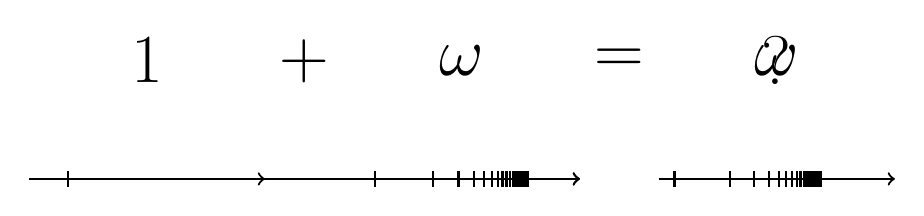
\begin{tikzpicture}
    \node at (0, 1.5) {\Huge $1$};
    \node at (2, 1.5) {\Huge $+$};
    \node at (4, 1.5) {\Huge $\omega$};
    \node at (6, 1.5) {\Huge $=$};
    \visible<-4>{\node at (8, 1.5) {\Huge ?};}
    \visible<5>{\node at (8, 1.5) {\Huge $\omega$};}

    \pause

    % draw the 1 line
    \visible<2>{\draw[thick, ->] (-1.5, 0) -- (1.5, 0);}
    \draw[thick] (-1, -0.1) -- (-1, 0.1);

    % draw the omega line
    \visible<2>{\draw[thick, ->] (2.5, 0) -- (5.5, 0);}
    \foreach \x in {1,...,20}
      \draw[thick] ({5.4 - 2.5 / sqrt(\x)}, -0.1) -- ({5.4 - 2.5 / sqrt(\x)}, 0.1);

    \pause
    % draw a line going through both the 1 and omega line
    \draw[thick, ->] (-1.5, 0) -- (5.5, 0);

    \pause
    \draw[thick, ->] (6.5, 0) -- (9.5, 0);
    \foreach \x in {1,...,20}
      \draw[thick] ({9.1 - 2.4 / sqrt(\x)}, -0.1) -- ({9.1 - 2.4 / sqrt(\x)}, 0.1);
    \pause
  \end{tikzpicture}
\end{frame}

\begin{frame}
  \frametitle{Non-commutativity of addition}
  \begin{figure}
    \centering

    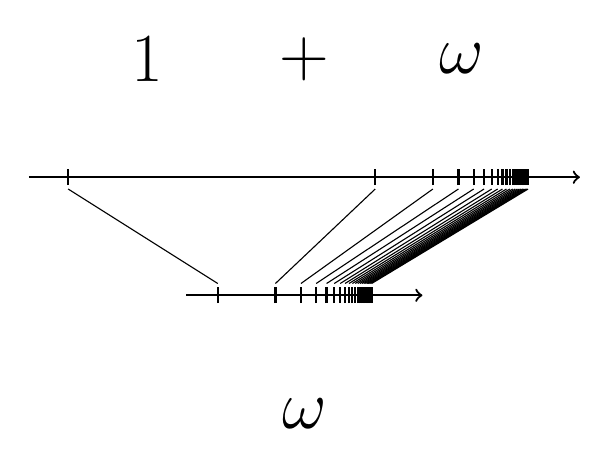
\begin{tikzpicture}
      \node at (0, 1.5) {\Huge $1$};
      \node at (2, 1.5) {\Huge $+$};
      \node at (4, 1.5) {\Huge $\omega$};
      \node at (2, -3) {\Huge $\omega$};

      % draw the 1+omega line
      \draw[thick, ->] (-1.5, 0) -- (5.5, 0);

      \draw[thick] (-1, -0.1) -- (-1, 0.1);

      \foreach \x in {1,...,20}
        \draw[thick] ({5.4 - 2.5 / sqrt(\x)}, -0.1) -- ({5.4 - 2.5 / sqrt(\x)}, 0.1);

      % draw the omega line underneath

      \draw[thick, ->] (0.5, -1.5) -- (3.5, -1.5);
      \foreach \x in {1,...,21}
        \draw[thick] ({3.4 - 2.5 / sqrt(\x)}, -1.6) -- ({3.4 - 2.5 / sqrt(\x)}, -1.4);

      \pause

      \draw (-1, -0.15) -- (0.9, -1.35);

      \pause
      \draw (2.9, -0.15) -- ({3.4 - 2.5 / sqrt(2)}, -1.35);

      \pause
      \draw ({5.4 - 2.5 / sqrt(2)}, -0.15) -- ({3.4 - 2.5 / sqrt(3)}, -1.35);

      \pause
      \foreach \x in {4,...,21}
        \draw ({5.4 - 2.5 / sqrt(\x-1)}, -0.15) -- ({3.4 - 2.5 / sqrt(\x)}, -1.35);
    \end{tikzpicture}
  \end{figure}
\end{frame}

\begin{frame}
  \frametitle{Non-commutativity of addition}
  \begin{center}
    \Huge $1 + \omega = \omega$
  \end{center}
\end{frame}

\begin{frame}
  \frametitle{Non-commutativity of addition}

  \begin{figure}
    \centering
    \begin{tikzpicture}
      \node at (0, 1.5) {\Huge $\omega$};
      \node at (2, 1.5) {\Huge $+$};
      \node at (4, 1.5) {\Huge $1$};
      \node at (2, -3) {\Huge $\omega$};

      % draw the omega+1 line
      \draw[thick, ->] (-1.5, 0) -- (5.5, 0);

      \draw[thick,color=red] (5, -0.1) -- (5, 0.1);

      \foreach \x in {1,...,20}
        \draw[thick] ({4.5 - 5 / sqrt(\x)}, -0.1) -- ({4.5 - 5 / sqrt(\x)}, 0.1);

      % draw the omega line underneath

      \draw[thick, ->] (-1.5, -1.5) -- (5.5, -1.5);
      \foreach \x in {1,...,21}
        \draw[thick] ({5 - 6 / sqrt(\x)}, -1.6) -- ({5 - 6 / sqrt(\x)}, -1.4);

      \pause

      \draw (5, -0.15) -- ({5 - 6 / sqrt(15)}, -1.35);

      \pause

      \draw (6, -0.15) -- ({5 - 6 / sqrt(16)}, -1.35);
      \node at (6.5, 0.5) {\Huge ?};
    \end{tikzpicture}
  \end{figure}
\end{frame}

\begin{frame}
  \frametitle{Non commutativity of addition}
  \begin{center}
    \Huge $\omega + 1 \neq \omega$ \\
    \pause \Huge $1+\omega = \omega$ \\
    \pause \Huge $1 + \omega \neq \omega + 1$
  \end{center}
\end{frame}

\section{The Hydra game}

\end{document}
